% This document provides the style to be used for a MSc Thesis at the
% Parallel and Distributed Systems group
\documentclass[11pt,twoside,a4paper,openright]{report}

% math packages
\usepackage{amsmath}
\usepackage{amssymb}

% textblocks for title page
\usepackage[absolute]{textpos}

% use babel for proper hyphenation
\usepackage[british]{babel}

% Graphics: different for pdflatex or dvi output, choose one
%%\usepackage[dvips]{graphicx}
%%\usepackage[pdftex]{graphicx}
\usepackage{graphicx}

\usepackage{epstopdf}
\usepackage{rotating}
\usepackage{subfigure}

% FONT
\usepackage[scaled=.92]{helvet}
%\usepackage{times}

% for url's use "\url{http://www.google.com/}"
\usepackage{url}
\usepackage[plainpages=false]{hyperref}



\usepackage{enumitem}

\usepackage{tikz}
\usetikzlibrary{positioning,arrows}

\tikzset{
  block/.style={
    draw,
    rectangle,
    minimum height=1cm,
    minimum width=1cm,
    align=center
  },
  subblock/.style={
    draw,
    rectangle,
    minimum height=.75cm,
    minimum width=1.5cm,
    align=center
  },
  line/.style={->,>=latex},
  XOR/.style={draw,circle,append after command={
        [shorten >=\pgflinewidth, shorten <=\pgflinewidth,]
        (\tikzlastnode.north) edge (\tikzlastnode.south)
        (\tikzlastnode.east) edge (\tikzlastnode.west)
        }
    }
}









% Information that will be filled in at various points in the report
\newcommand{\reportTitle}{Leveraging VLC for energy disaggregation in Smart Buildings}
\newcommand{\reportAuthor}{Johnny Verhoeff}
\newcommand{\reportEmail}{j.s.c.j.verhoeff@student.tudelft.nl}
\newcommand{\reportUrlEmail}{\href{mailto:\reportEmail}{\reportEmail}}
\newcommand{\reportMSC}{Embedded Systems} %{Embedded Systems}{Computer Engineering}{Computer Science}{Electrical Engineering}
\newcommand{\reportDate}{\today} %TODO: Dit is de datum van uitgifte van final versie aan de afstudeer commissie
\newcommand{\presentationDate}{\today} %TODO: Dit is de datum van de afstudeerpresentatie
\newcommand{\graduationCommittee}{
TODO GRADUATION COMMITTEE & Delft University of Technology \\
TODO GRADUATION COMMITTEE & Delft University of Technology \\
} % The order of listing the names: Graduation prof, supervisor(s), others ordered by title + alphabetical
%examples:
%prof. dr. ir. H. J. Sips (chair) & Delft University of Technology \\
%ir. dr. D. H. J. Epema           & Delft University of Technology \\
\newcommand{\reportAbstract}{TODO ABSTRACT}
\newcommand{\reportKeywords}{VLC, CDMA}

% For pdflatex
\pdfinfo{
   /Author (\reportAuthor)
   /Title  (\reportTitle)
   /Keywords (\reportKeywords)
}

\begin{document}

\pagenumbering{alph}
\pagestyle{empty}


% FRONTCOVER
%%\usepackage[total={210mm,297mm},left=0pt,bottom=0pt,top=0cm,right=0pt,headsep=0pt,head=0pt,showframe]{geometry}

%%\input{preambleL31958}
%%\begin{titlepage}
\begin {textblock*}{210mm}(0mm,0mm)
\noindent

\includegraphics[height=3.2cm]{pics/block}
\sffamily
\vspace{.8cm}
\begin{center}
\Large
Delft University of Technology\\
Master's Thesis in \reportMSC\\
\vspace{2cm}
\parbox{170mm}{\bfseries\centering\Huge\reportTitle}\\
\vspace{1cm}
\parbox{170mm}{\bfseries\centering\reportAuthor}

\end{center}
\end{textblock*}

\begin {textblock*}{210mm}[0.0,1.0](0mm,297mm)
\noindent
\hspace{1.89cm}


\hfill\parbox{5cm}{

\includegraphics[width=5cm]{pics/es_logo_cyan_black_rgb}}
\hspace*{2cm}\\

\vspace*{1.5cm}
\noindent

\includegraphics[width=\textwidth]{pics/TU_border_A4_L_front}
\end{textblock*}

\null\newpage


%%%%%%%%%%%%%%%%%%%%%%%%%%%%%%%%%%%%%%%%%%%%%%%%%%%%%%%%%%%%%%%%%%%%%%%%%%%%%%%
\hoffset=1.63cm
\oddsidemargin=0in
\evensidemargin=0in
\textwidth=5in

%%%%%%%%%%%%%%%%%%%%%%%%%%%%%%%%%%%%%%%%%%%%%%%%%%%%%%%%%%%%%%%%%%%%%%%%%%%%%%%
\parindent=1em

% EMPTY PAGE
\cleardoublepage

\pagestyle{plain}
\pagenumbering{roman}
\setcounter{page}{1}

% TITLE PAGE: page i (hidden)
\begin{titlepage}

  \begin{center}
  \null\vfill
    \begin{center}
    \LARGE{\reportTitle}
    \end{center}

    \vspace{3cm}

    \begin{large}
    Master's Thesis in \reportMSC
    \end{large}

    \vspace{1.5cm}

    \begin{normalsize}
    Embedded Software Section\\
    Faculty of Electrical Engineering, Mathematics and Computer Science\\
    Delft University of Technology\\
    Mekelweg 4, 2628 CD Delft, The Netherlands
    \end{normalsize}

    \vspace{2.0cm}

    \begin{normalsize}
    \reportAuthor \\
    \reportUrlEmail
    \end{normalsize}

    \vspace{1.0cm}

    % <MM> DD, YYYY
    \reportDate             %TODO: Dit is de datum van uitgifte van final versie aan de afstudeer commissie

  \vfill
  \end{center}

\end{titlepage}


% GRADUATION DATA AND ABSTRACT: pages ii and iii (hidden)
%De aankondiging bevat de spreker, titel, plaats, datum en tijd, samenstelling van de afstudeercommissie en een korte samenvatting (maximaal 25 regels).
\thispagestyle{empty}

\noindent \textbf{Author}\\
\begin{tabular}{l}
\reportAuthor{} (\reportUrlEmail)\\
\end{tabular}\\
\noindent \textbf{Title}\\
\begin{tabular}{l}
\reportTitle\\
\end{tabular}\\
\noindent \textbf{MSc presentation}\\
\begin{tabular}{l}
% <MM> DD, YYYY (like \today)
\presentationDate\\
\end{tabular}

\vspace{1.1cm}

\noindent \textbf{Graduation Committee}\\
\begin{tabular}{ll}
\graduationCommittee
\end{tabular}


\begin{abstract} %de abstract bevat alleen een korte samenvatting van de inhoud van het onderzoek
\setcounter{page}{3}
\reportAbstract{}
\end{abstract}

\clearpage

%\setcounter{page}{4}

% EMPTY PAGE: page iv
\cleardoublepage

% OPTIONAL QUOTATION: page v
%\pagestyle{empty}

\null\vfill

\begin{center}
\emph{``TODO QUOTE''} -- TODO QUOTED PERSON
\end{center}

\vspace{10cm}

\clearpage


% EMPTY PAGE: page vi
%\cleardoublepage

% PREFACE: page v
% !TeX root = ../thesis.tex

\chapter*{Preface}
\addcontentsline{toc}{chapter}{Preface}



This Master thesis is the final part of the Master of Science in Embedded Systems program I followed at Delft University of Technology.
Prior to this thesis, I had little knowledge of VLC or energy disaggregation.
Using VLC in combination with energy disaggregation has not been explored yet.
The first steps towards disaggregating individual lights are taken in this thesis.
There are experimental results achieved as well as theoretical results, through simulation.







\vspace{1\baselineskip}

\noindent



First, I would like to thank my loving family, who have support me throughout this nine-month thesis project.
I would also like to thank my advisor Marco Z\'u\~niga Zamalloa and Akshay Narashiman for their guidance to help me finish my thesis.
Finally I want to acknowledge Koen Langendoen and Laura Ramirez Elizondo for being members of my graduation committee.







\vspace{1\baselineskip}

\noindent
Johnny Verhoeff

\vspace{1\baselineskip}

\noindent
Delft, The Netherlands

\noindent
\today

% EMPTY PAGE: page
\cleardoublepage

% TABLE OF CONTENTS: starting at page vii
\tableofcontents

\cleardoublepage

\pagenumbering{arabic}
\setcounter{page}{1}




% INTRODUCTION: page 1
\chapter{Introduction}
\label{chp:introduction}
TODO INTRODUCTION

\vspace{1\baselineskip}

\noindent
TODO ORGANISATIONAL DESCRIPTION OF THESIS



% CHAPTERS ... For instance: History/Prior Work, Design/Implementation, Experiments
\chapter{CHAPTER TITLE}
\label{chp:CHAPTERTITLE}
INTRODUCTION TEXT TO THIS CHAPTER IN WHICH ALL SECTIONS ARE DESCRIBED ROUGHLY (1 SENTENCE EACH).

This chapter describes the ... In Section~\ref{sec:SECTIONTITLE}, examples are given of how to use tables and figures in MSc theses.

\section{SECTION TITLE}
\label{sec:SECTIONTITLE}

Every caption of a table (or figure) should start with a capital letter, and should end with a period. References to tables are given with a capital letter for table, as in ``(see Table~\ref{tab:EXAMPLETABLE})'' or ``in Table~\ref{tab:EXAMPLETABLE}, ...''.

\begin{table}[htb]
\centering
\begin{tabular}{|l|c|r|}
\hline % horizontal line
left aligned & centred & right aligned \\
\hline \hline
12           & 34      & 56            \\
\hline
\end{tabular}
\caption{Complete sentence describing the tabular data.}
\label{tab:EXAMPLETABLE}
\end{table}

References to figures are given with a capital letter for figure, as in ``(see Figure~\ref{fig:EXAMPLEFIGURE})'' or ``in Figure~\ref{fig:EXAMPLEFIGURE}, ...''.

\cite{b}
\cite{a}

\begin{figure}[htb]
% most GNUplot figures need to be rotated, width should be the same throughout the complete document, and no extension is needed

\includegraphics[angle=180,width=\textwidth]{pics/TUD_logo_zw}
\caption{Complete sentence describing the figure thoroughly.}
\label{fig:EXAMPLEFIGURE}
\end{figure}



%!TEX root = ../../thesis.tex

\section{CDMA}
\label{sec:CDMA}

	This section will explain what CDMA is, alternatives and why it is needed.

	When transmitting data from a transmitter to a receiver over a channel, the entire channel is being used for this purpose.
	If one wants to have multiple transmitters transmitting over one channel, there is a problem. 
	The transmitters interfere with each other, this is called multiple access interference (MAI). 
	There are several ways to get around this problem: 

	\begin{itemize}
		\item TDM: Time Division Multiplexing. \\
				Each transmitter gets assigned a time slot, in which it and only it is allowed to transmit, hereby going around the MAI problem.
		\item FDM: Frequency Division Multiplexing. \\
				Each transmitters gets assigned a frequency band. Each transmitter is allowed to transmit the whole time, but only at the assigned frequencies.
		\item CDM: Code Division Multiplexing. \\
				Each transmitter gets assigned a code word. 
				The data first needs to be encoded using the code word and then the transmitter can send his message. 
				Each transmitter can transmit all the time using the entire frequency band. 
				These codes will determine how many transmitters can actually transmit with correct decoding results at the receiver end.
	\end{itemize}

	The distributed network of the VLC LEDs is inherently uncoordinated, since all the LEDs are basically only lights. 
	They have no receiver of any kind. 
	They can only implicitly transmit data by turning the load or the LED on or off.
	Because the LEDs cannot receive data, they cannot be assigned a time slot and therefor we cannot use a TDM scheme.

	An FDM scheme is also not applicable.
	This is because the LEDs do not have an explicit hardware transmitter that can modulate a signal.
	Instead the transmitting is implicitly done via turning the LED on and off.
	So only binary values of the current draw are sent as signals.

	This is where the CDM approach comes into play.
	This scheme allows the multiple LEDs to transmit at the same time.
	But the type of code used here is of importance.
	The code type determines the MAI and what the receiver is able to decode.

	\subsection{Performance metrics of a code}
	\label{subsec:performance-metrics}

		To determine which code is the best for this problem some measures are needed to be able to compare the codes.

		One such a measure is called the correlation.
		Correlation is a measure for determining how much sequence $X$ is similar to sequence $Y$ and can be found in \autoref{eq:correlation}.
		With $L$ being the length of the code and $\tau$ the time-shift.
		When sequence $X$ and $Y$ are the same sequence, we speak of the autocorrelation.
		When they are two different sequences, we speak of the cross-correlation. 

		\begin{equation}
			R(\tau)_{xy} = \displaystyle\sum_{i = 0} ^ {L - 1} x(i) \times y(i + \tau) {\text{  with $\tau = 0, 1, 2, \dotsc, L$}}
			\label{eq:correlation}
		\end{equation}

		The properties of an ideal code set should be, that the autocorrelation for each code in the set should be $0$ for each time-shift $\tau \neq 0$, at $\tau = 0$ the autocorrelation should be $L$.
		The ideal cross-correlation properties should $0$ for every time-shift $\tau$, so that no code interferes with any other code, hereby causing no MAI.

		Other metrics to be considered are the length of the code and how many codes there are in that code set.
		The code length is of importance because each bit a user will transmit must be encoded. 
		So the the message that will be transmitted via the channel will be the length of the code times the length of the data.
		If there are only a few codes in a code set then only a few number of users can transmit which does not scale well. 

	\subsection{Walsh-Hadamard Sequences}

		Walsh-Hadamard sequences are sequences which are created using a Hadamard matrix.
		Hadamard matrices are $n \times n$ matrices which are recursively generated.
		Starting with a $1 \times 1$ matrix: 
		$H_{1} = \begin{bmatrix} 1 \end{bmatrix}$, then 
		$H_{2} = \begin{bmatrix} 1 & 1 \\ 1 & -1 \end{bmatrix}$.
		Or in general: $H_{2n} = \begin{bmatrix} H_n & H_n \\ H_n & -H_n \end{bmatrix}$ \cite{714616}.
		The matrix can also be filled with binary values: zero and one. In that case the general matrix will be: 
		$H_{2n} = \begin{bmatrix} H_n & H_n \\ H_n & \overline{H_n} \end{bmatrix}$

		The Hadamard matrix has the property that every row in the matrix is orthogonal to every other row.
		Hadamard matrices exist for every power of $2$, so the code length is also a power of $2$.
		So for $\tau = 0$, the cross-correlation is $0$, but when $\tau \neq 0$ not all the rows are orthogonal anymore.
		\cite{1182447} proved that an Hadamard matrix of size $2^P$ could be divided into $P + 1$ subsets of rows, where one code could be selected giving $P + 1$ orthogonal codes for each time-shift $\tau$.
		These codes are called Cyclically Orthogonal Walsh Hadamard Codes (COWHC).

		All rows of the matrix have the property that the autocorrelation at $\tau = 0$ is equal to $L$.
		But when $\tau \neq 0$, undesirable behavior occurs as can be seen in \autoref{fig:autocorr-hadamard}.
		The autocorrelation function has several high peaks where only one is desired.
		This means that if a transmitter sends an encoded message with this code and the receiver does not know when in time the start of the message is, the receiver would get false positives for data.

		\begin{figure}
			\centering
			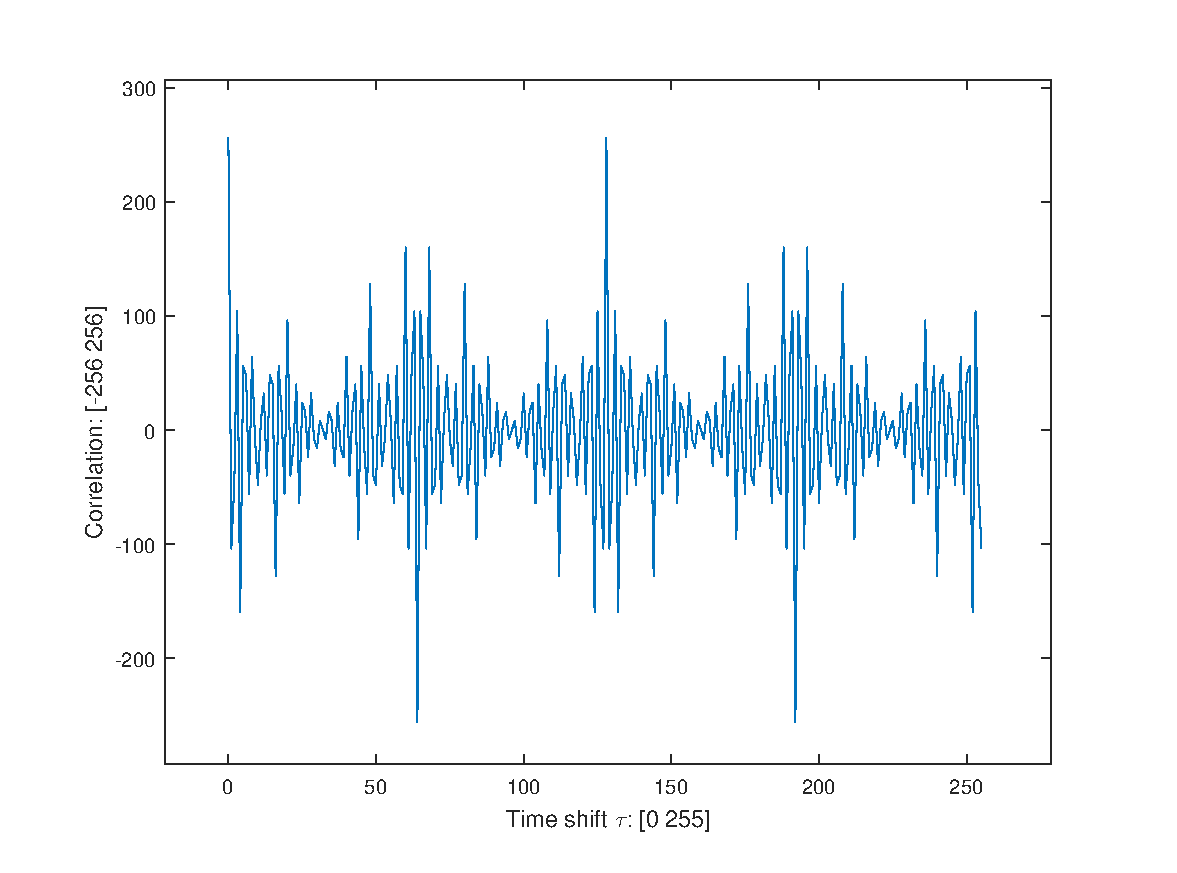
\includegraphics[width=\textwidth]{chapters/CDMA/autocorr-hadamard.eps}
			\caption{Autocorrelation of Hadamard code with index 120 of length 256.}
			\label{fig:autocorr-hadamard}
		\end{figure}

		So only a small subset of the codes have $0$ cross-correlation for every time-shift $\tau$ and the autocorrelation is far from what the ideal code set should have.


	\subsection{PN Sequences}

		PN sequences are sequences where the numbers looks like they are randomly generated but they are easily generated in software or hardware.
		The sequences have the following noise-like properties~\cite{mitra2008pseudo}:

		\begin{itemize}
			\item Balanced \\
					Any PN sequence of length $L = 2^n - 1$ contains exactly $2^{n-1}$ ones and $2^{n-1} - 1$ zeros.

			\item Runs \\
					A run is a subset of the sequence where all the consecutive numbers are the same.
					In any PN sequence, $1/2$ of the runs have length 1, $1/4$ have length 2, $1/8$ have length 3 and so on.

			\item Autocorrelation \\
					The autocorrelation function of a PN sequence will take on two values as can be seen in \autoref{eq:autocorr-pn} and \autoref{fig:autocorr-pn}.


		\end{itemize}

		\begin{equation}
			\label{eq:autocorr-pn}
			R(\tau) = 
				\begin{cases}
					L    & \quad \text{if } \tau = 0 \\
					-1   & \quad \text{if } \tau \neq 0 \\
				\end{cases}
		\end{equation}

		\begin{figure}
			\centering
			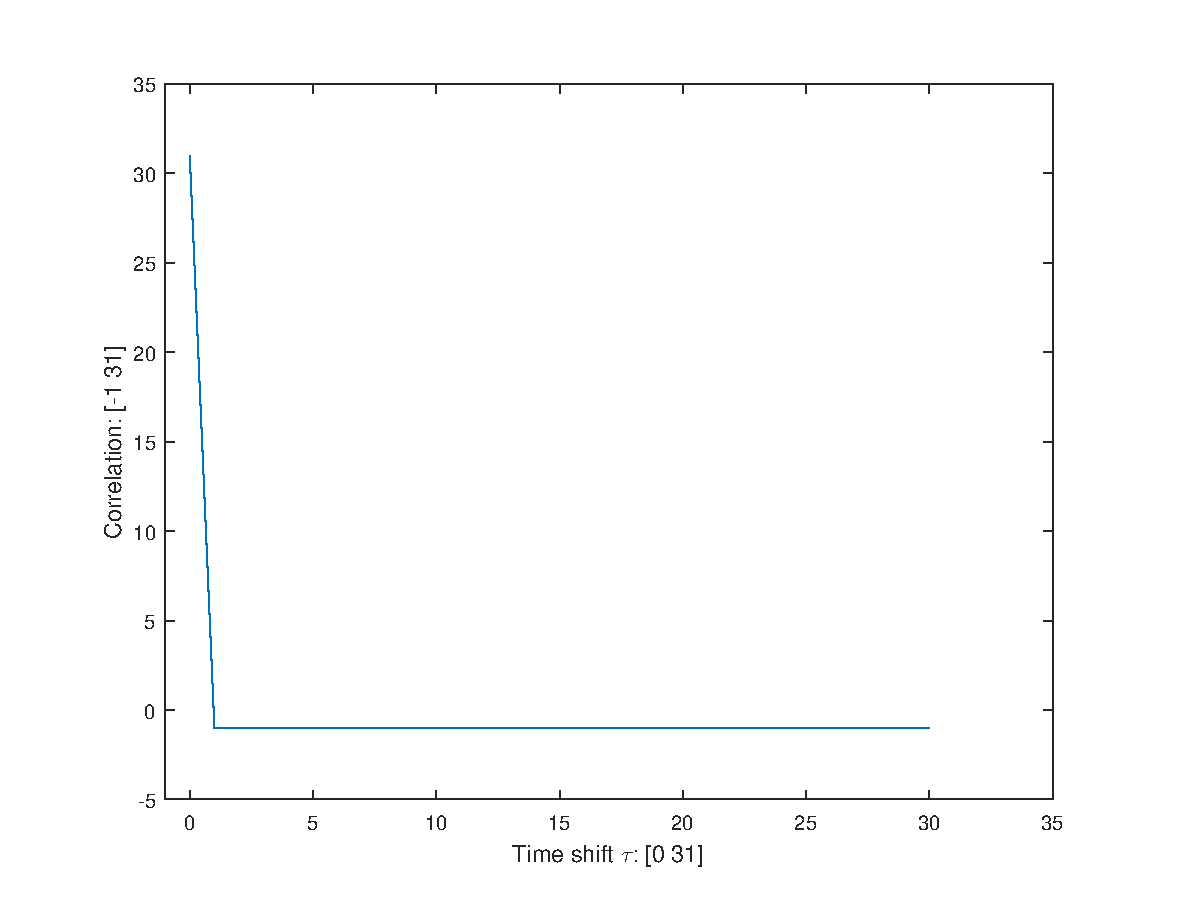
\includegraphics[width=\textwidth]{chapters/CDMA/autocorr-pn.eps}
			\caption{Autocorrelation of PN sequence of length 31.}
			\label{fig:autocorr-pn}
		\end{figure}

		PN sequences are generated using a linear feedback shift register (LFSR) \cite{Wang:1988:LFS:52007.52024}.
		\autoref{fig:lfsr} shows an $n$ length LFSR with some XOR gates attached to it.
		The LFSR is defined entirely by the feedback function, also called a characteristic polynomial.
		It determines the length and the type of sequence generated.
		The polynomial looks like \autoref{eq:lfsr-polynomial}.
		The LFSR in \autoref{fig:lfsr} contains $n$ shift registers and is initiated with a starting seed.
		This seed can be any vector apart from the all zero vector.
		The reason for this is because the XOR function with two zeros as input will output a zero, making the sequence that this LFSR outputs a sequence of all zeros.
		The output of the shift registers are multiplied with the coefficients of the characteristic polynomial ($C_{n-1}, C{n-2}, \dotsc, C_1, C_0$).
		The result output is then fed back into the first shift register, all the bits in the rest of the registers also shift one position and one output bit is created.
		With $n$ number of registers and the zero start vector excluded it takes $2^n - 1$ steps to output the entire sequence before it starts to repeat itself.


		\begin{figure}
			\centering
			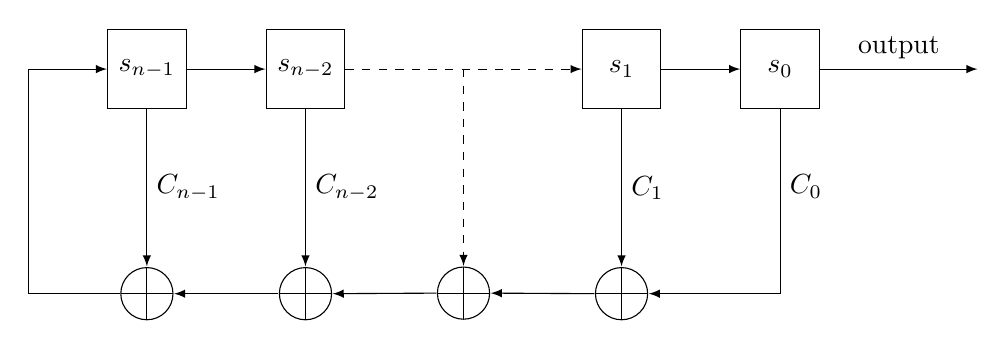
\begin{tikzpicture}


				\node[block                  ] (a) {$s_{n-1}$};
				\node[block, right = 1cm of a] (b) {$s_{n-2}$};
				\draw[line] (a.east) -- (b.west) ;

				\node[block, right = 3cm of b] (c) {$s_{1}$};
				\node[block, right = 1cm of c] (d) {$s_{0}$};
				\draw[line] (c.east) -- (d.west) ;

				\draw[dashed, line] (b.east) -- (c.west) ;

				\node[coordinate, right = 2cm of d] (e) {};
				\draw[line] (d.east) -- (e.west) node [midway, above] {output};

				\node[XOR, scale=2, below = 2cm of c] (f) {};
				\draw[line] (c.south) -- (f.north) node [midway, right] {$C_1$};
				\draw[line] (d.south) |- (f.east) node [pos=0.21, right] {$C_0$};

				\node[coordinate, right = 1.5cm of b] (h) {};
				\node[XOR, scale=2, below = 2.5cm of h] (g) {};
				\draw[line] (f.west) -- (g.east) ;
				\draw[dashed, line] (h.south) -- (g.north) ;

				\node[XOR, scale=2, below = 2cm of b] (i) {};
				\node[XOR, scale=2, below = 2cm of a] (k) {};

				\draw[line] (b.south) -- (i.north) node [midway, right] {$C_{n-2}$};
				\draw[line] (g.west) -- (i.east) ;
				
				\draw[line] (i.west) -- (k.east) ;
				\draw[line] (a.south) -- (k.north) node [midway, right] {$C_{n-1}$};

				\node[coordinate, left = 1cm of a] (j) {};
				
				\draw[line] (k.west) -| (j) -- (a.west) ;




			\end{tikzpicture}
			\caption{Linear feedback shifter register of length $n$, with XOR gates.}
			\label{fig:lfsr}
		\end{figure}

		\begin{equation}
			\label{eq:lfsr-polynomial}
			p(x) = x^n + C_{n-1} x^{n-1}  + C_{n-2} x^{n-2} + \dotsc + C_{2} x^{2}  + C_{1} x  + C_{0}
		\end{equation}


		% something about cross correlation....






		





%!TEX root = ../thesis.tex

\section{Encoding \& Decoding Data Simulation}
\label{sec:enc-dec-theory}

	All of the coding schemes as discussed in \autoref{sec:CDMA} are designed for wireless transceivers.
	Meaning they send a radio wave through the air which is encoded with that particular code sequence.
	That radio wave is an analog signal and can vary between $+1$ and $-1$ symbols.
	But the VLC enabled LEDs cannot send such signals.
	They can only be turned on or off, thus encoding only $0$ and $1$ symbols.
	Those symbols correspond to a current draw of the LED which is measured by an ADC for example.
	To experiment with the encoding and decoding process and obstacles without the need for hardware, we use Matlab to simulate the process.

	\subsection{Walsh-Hadamard Sequences}

		%about radio dec. and bin. enc. proof etc...
		The way the Walsh-Hadamard sequences work with encoding and decoding with for example the link from a base-station to a mobile device of a CDMA application, is that the sequence of $+1$ and $-1$ symbols gets multiplied with the encoded data. 
		Say for example that we have a Hadamard matrix of rank $8$ as can be seen in \autoref{matrix:h8} which is created by using \autoref{eq:hadamard-matrix-creation}.
		And we select a random code to encode our data with, which corresponds to a row of this matrix.
		We also assume that our data is binary, consisting of 0s and 1s. 
		Our last assumption is that is we want to encode a $0$ we use the code itself and if we want to encode a $1$ we use the inverse of the code, i.e. $-1 \times$ the code.
		That describes the encoding process. 
		The decoding process involves the calculation of the correlation of the received signal with a code sequence for which we want to know if there is information embedded in the received signal and if so, what might that information be.

			\begin{equation}
				H_8 = 
				\begin{bmatrix*}[r] 
					H_4 & H_4 \\ 
					H_4 & -H_4 
				\end{bmatrix*}
				%=
				%\begin{bmatrix*}[r] 
				%	H_2 & H_2   & H_2 & H_2   \\
				%	H_2 & -H_2  & H_2 & -H_2  \\
				%	H_2 & H_2   & -H_2 & -H_2 \\
				%	H_2 & -H_2  & -H_2 & H_2  \\
				%\end{bmatrix*}
				=
				\dotsc
				=
				\begin{bmatrix*}[r]
					1	&	 1	&	 1	&	 1	&	 1	&	 1	&	 1	&	 1 \\
					1	&	-1	&	 1	&	-1	&	 1	&	-1	&	 1	&	-1 \\
					1	&	 1	&	-1	&	-1	&	 1	&	 1	&	-1	&	-1 \\
					1	&	-1	&	-1	&	 1	&	 1	&	-1	&	-1	&	 1 \\
					1	&	 1	&	 1	&	 1	&	-1	&	-1	&	-1	&	-1 \\
					1	&	-1	&	 1	&	-1	&	-1	&	 1	&	-1	&	 1 \\
					1	&	 1	&	-1	&	-1	&	-1	&	-1	&	 1	&	 1 \\
					1	&	-1	&	-1	&	 1	&	-1	&	 1	&	 1	&	-1 
				\end{bmatrix*}
				\label{matrix:h8}
			\end{equation}

		Since the autocorrelation of Walsh-Hadamard sequences do not allow to find the beginning of a code, see \autoref{fig:autocorr-hadamard}, we will only consider the synchronized situation, for which these codes are also used in practice, so $\tau = 0$.
		Say we have a code $c_i(t)$ and we want to encode a $0$ with this code and send that as a signal for our receiver to receive.
		The receiver will receive this signal $s(t)$ assuming a perfect channel, the decoding process can be seen below.

		%Want something different than proof, but dont know how/what

		\begin{proof}
			Let $s(t)$ be the received signal which encodes a 0 for code: $c_i(t)$.\\
			And let $c_i(t)$ be the code for which we want to check if there is information there. \\

			\begin{align*}
				R(\tau)_{xy} = \displaystyle\sum_{t = 0} ^ {L - 1} x(t) \times y(t + \tau)	\tag{See \autoref{eq:correlation}}
				\\ \tau = 0,\ x = s(t),\ y = c_i(t)	
				\\ R(0)_{sc_{i}} = \displaystyle\sum_{t = 0} ^ {L - 1} s(t) \times c_i(t)	
				\\ s(t) = c_i(t)															
				\\ R(0)_{sc_{i}} = \displaystyle\sum_{t = 0} ^ {L - 1} c_i(t) \times c_i(t) = L
			\end{align*}

		\end{proof}

		We can also state what the result will be when we decode a $1$ with a code $c_i(t)$, see below:

		\begin{proof}
			Let $s(t)$ be the received signal which encodes a 1 for code: $c_i(t)$.\\
			And let $c_i(t)$ be the code for which we want to check if there is information there. \\

			\begin{align*}
				R(\tau)_{xy} = \displaystyle\sum_{t = 0} ^ {L - 1} x(t) \times y(t + \tau)	\tag{See \autoref{eq:correlation}}
				\\ \tau = 0,\ x = s(t),\ y = c_i(t)	
				\\ R(0)_{sc_{i}} = \displaystyle\sum_{t = 0} ^ {L - 1} s(t) \times c_i(t)	
				\\ s(t) = -1 \times c_i(t)															
				\\ R(0)_{sc_{i}} = \displaystyle\sum_{t = 0} ^ {L - 1} -1 \times c_i(t) \times c_i(t)
				\\ &= -1 \times \displaystyle\sum_{t = 0} ^ {L - 1} c_i(t) \times c_i(t) = -1 \times L
			\end{align*}

		\end{proof}

		This two statement state that if we encode a data bit with code $c_i$ and that is the only information received by the receiver, we either get the maximum positive correlation, i.e. $L$ or we get the maximum negative correlation, i.e. $-L$.
		If we would have received a signal consisting of only zeros the correlation would also be zero.

		Next let us look at what happens when we try to decode information with a different code than the code which was used to encode information with. In that case we also get a correlation of zero, see below. This is per definition the case since we are using Walsh-Hadamard codes which are orthogonal to each other when they are synchronized.

		\begin{proof}
			Let $s(t)$ be the received signal which encodes a data bit for code: $c_i(t)$.\\
			And let $c_j(t)$ be the code for which we want to check if there is information there. \\

			\begin{align*}
				R(\tau)_{xy} = \displaystyle\sum_{t = 0} ^ {L - 1} x(t) \times y(t + \tau)	\tag{See \autoref{eq:correlation}}
				\\ \tau = 0,\ x = s(t),\ y = c_j(t)	
				\\ R(0)_{sc_{i}} = \displaystyle\sum_{t = 0} ^ {L - 1} s(t) \times c_j(t)	
				\\ s(t) = c_i(t)															
				\\ R(0)_{sc_{i}} = \displaystyle\sum_{t = 0} ^ {L - 1} c_i(t) \times c_j(t) = 0
			\end{align*}

		\end{proof}

		Finally we look at the decoding process for when the received signal consists of several encoded signals, see below. 
		Because all the codes in Walsh-Hadamard sequences are orthogonal to each other they produce no MAI and so there can be as many codes superimposed on each other and still a correct decoding can take place. 


		\begin{proof}
			Let $s(t)$ be the received signal which encodes data for several codes: $c_i(t)$, $c_j(t)$, $c_k(t)$ and $c_l(t)$.\\
			And let $c_i(t)$ be the code for which we want to check if there is information there. \\

			\begin{align*}
				R(\tau)_{xy} = \displaystyle\sum_{t = 0} ^ {L - 1} x(t) \times y(t + \tau)	\tag{See \autoref{eq:correlation}}
				\\ \tau = 0,\ x = s(t),\ y = c_i(t)	
				\\ R(0)_{sc_{i}} = \displaystyle\sum_{t = 0} ^ {L - 1} s(t) \times c_i(t)	
				\\ s(t) = c_i(t) + c_j(t) + c_k(t) + c_l(t)															
				\\ R(0)_{sc_{i}} = \displaystyle\sum_{t = 0} ^ {L - 1} \{ c_i(t) + c_j(t) + c_k(t) + c_l(t) \} \times c_i(t)
				\\ R(0)_{sc_{i}} = \displaystyle\sum_{t = 0} ^ {L - 1} c_i(t) \times c_i(t) + c_j(t) \times c_i(t) + c_k(t) \times c_i(t) + c_l(t) \times c_i(t)
				\\ = L + 0 + 0 + 0 = L
			\end{align*}

		\end{proof}

		But as stated in \autoref{sec:enc-dec-theory} the VLC enabled LEDs cannot send $+1$ and $-1$ symbols of data, they can only be in an on or off state.
		This means that the code that is being used for encoding must be mapped to zeros and ones.
		Let us assume that a $+1$ symbol maps to an off state, i.e. $0$ and that a $-1$ symbol maps to an on state, i.e. $1$.
		We can summarize that in \autoref{eq:radio-to-bin}, where $r$ denotes the $+1$ or $-1$ symbols and the outcome $b$ will be our binary value, i.e. $0$ or $1$.

		\begin{equation}
			b = \frac{1 - r}{2}
			\label{eq:radio-to-bin}
		\end{equation}

		Because we are now using the binary values as code, we can no longer use multiply to encode our binary information.
		Instead, we must use th XOR function.
		Now let us see what happens when we try to decode information that has been encoded using on-off keying (OOK), below is stated what happens when both data bits are encoded.

		\begin{proof}
			Let $s(t)$ be the received signal which encodes a 0 for code: $c^b_i(t)$, where $c^b_i(t)$ is binary valued, i.e. $0$ or $1$ \\
			And let $c^r_i(t)$ be the code for which we want to check if there is information there, where $c^r_i(t)$ uses the traditional values $-1$ and $+1$ \\

			\begin{align*}
				R(\tau)_{xy} = \displaystyle\sum_{t = 0} ^ {L - 1} x(t) \times y(t + \tau)	\tag{See \autoref{eq:correlation}}
				\\ \tau = 0,\ x = s(t),\ y = c^r_i(t)	
				\\ R(0)_{sc^r_{i}} = \displaystyle\sum_{t = 0} ^ {L - 1} s(t) \times c^r_i(t)	
				\\ s(t) = \forall t \in \{ 0, 1, 2, \dotsc, L - 1 \} \ \ 0(t) \oplus c^b_i(t) = c^b_i(t) \tag{Where $0(t) = 0 \ \forall t$ }										
				\\ R(0)_{sc^r_{i}} = \displaystyle\sum_{t = 0} ^ {L - 1} c^b_i(t) \times c^r_i(t)
				\\ = \displaystyle\sum_{t = 0} ^ {L - 1} \frac{1 - c^r_i(t)}{2} \times c^r_i(t) \tag{Via \autoref{eq:radio-to-bin}}
				\\ = \frac{1}{2} \times \displaystyle\sum_{t = 0} ^ {L - 1} c^r_i(t) - c^r_i(t) \times c^r_i(t)
				\\ = \frac{1}{2} \times \displaystyle\sum_{t = 0} ^ {L - 1} c^r_i(t) - \frac{1}{2} \times \displaystyle\sum_{t = 0} ^ {L - 1} c^r_i(t) \times c^r_i(t)
				\\ = 0 - \frac{1}{2} \times \displaystyle\sum_{t = 0} ^ {L - 1} c^r_i(t) \times c^r_i(t) \tag{Balance property}
				\\ = - \frac{1}{2} \times L
			\end{align*}

		\end{proof}

		\begin{proof}
			Let $s(t)$ be the received signal which encodes a 1 for code: $c^b_i(t)$, where $c^b_i(t)$ is binary valued, i.e. $0$ or $1$ \\
			And let $c^r_i(t)$ be the code for which we want to check if there is information there, where $c^r_i(t)$ uses the traditional values $-1$ and $+1$ \\

			\begin{align*}
				R(\tau)_{xy} = \displaystyle\sum_{t = 0} ^ {L - 1} x(t) \times y(t + \tau)	\tag{See \autoref{eq:correlation}}
				\\ \tau = 0,\ x = s(t),\ y = c^r_i(t)	
				\\ R(0)_{sc^r_{i}} = \displaystyle\sum_{t = 0} ^ {L - 1} s(t) \times c^r_i(t)	
				\\ s(t) = \forall t \in \{ 0, 1, 2, \dotsc, L - 1 \} \ \ 1(t) \oplus c^b_i(t) = 1 - c^b_i(t) \tag{Where $1(t) = 1 \ \forall t$ }
				\\ R(0)_{sc^r_{i}} = \displaystyle\sum_{t = 0} ^ {L - 1} (1 - c^b_i(t)) \times c^r_i(t)
				\\ = \displaystyle\sum_{t = 0} ^ {L - 1} (1 - \frac{1 - c^r_i(t)}{2}) \times c^r_i(t) \tag{Via \autoref{eq:radio-to-bin}}
				\\ = \displaystyle\sum_{t = 0} ^ {L - 1} \frac{1 + c^r_i(t)}{2} \times c^r_i(t)
				\\ = \frac{1}{2} \times \displaystyle\sum_{t = 0} ^ {L - 1} c^r_i(t) + c^r_i(t) \times c^r_i(t)
				\\ = \frac{1}{2} \times \displaystyle\sum_{t = 0} ^ {L - 1} c^r_i(t) + \frac{1}{2} \times \displaystyle\sum_{t = 0} ^ {L - 1} c^r_i(t) \times c^r_i(t)
				\\ = 0 + \frac{1}{2} \times \displaystyle\sum_{t = 0} ^ {L - 1} c^r_i(t) \times c^r_i(t) \tag{Balance property}
				\\ = \frac{1}{2} \times L
			\end{align*}

		\end{proof}

		The case for when there is no data encoded for this particular code:

		\begin{proof}
			Let $s(t)$ be the received signal which encodes data for code: $c^b_i(t)$, where $c^b_i(t)$ is binary valued, i.e. $0$ or $1$ \\
			And let $c^r_j(t)$ be the code for which we want to check if there is information there, where $c^r_j(t)$ uses the traditional values $-1$ and $+1$ \\

			\begin{align*}
				R(\tau)_{xy} = \displaystyle\sum_{t = 0} ^ {L - 1} x(t) \times y(t + \tau)	\tag{See \autoref{eq:correlation}}
				\\ \tau = 0,\ x = s(t),\ y = c^r_j(t)	
				\\ R(0)_{sc^r_{i}} = \displaystyle\sum_{t = 0} ^ {L - 1} s(t) \times c^r_j(t)	
				\\ s(t) = c^b_i(t)										
				\\ R(0)_{sc^r_{i}} = \displaystyle\sum_{t = 0} ^ {L - 1} c^b_i(t) \times c^r_j(t)
				\\ = \displaystyle\sum_{t = 0} ^ {L - 1} \frac{1 - c^r_i(t)}{2} \times c^r_j(t) \tag{Via \autoref{eq:radio-to-bin}}
				\\ = \frac{1}{2} \times \displaystyle\sum_{t = 0} ^ {L - 1} c^r_j(t) - c^r_i(t) \times c^r_j(t)
				\\ = \frac{1}{2} \times \displaystyle\sum_{t = 0} ^ {L - 1} c^r_j(t) - \frac{1}{2} \times \displaystyle\sum_{t = 0} ^ {L - 1} c^r_i(t) \times c^r_j(t)
				\\ = 0 - \frac{1}{2} \times \displaystyle\sum_{t = 0} ^ {L - 1} c^r_i(t) \times c^r_i(t) \tag{Balance property}
				\\ = 0 + 0 = 0\tag{Because the codes are orthogonal.}
			\end{align*}

		\end{proof}

		Finally the case for when there are multiple signals:


		\begin{proof}
			Let $s(t)$ be the received signal which encodes data for several codes: $c^b_i(t)$, $c^b_j(t)$, $c^b_k(t)$ and $c^b_l(t)$, where $c^b_i(t)$ is binary valued, i.e. $0$ or $1$\\
			And let $c^r_i(t)$ be the code for which we want to check if there is information there, where $c^r_i(t)$ uses the traditional values $-1$ and $+1$ \\

			\begin{align*}
				R(\tau)_{xy} = \displaystyle\sum_{t = 0} ^ {L - 1} x(t) \times y(t + \tau)	\tag{See \autoref{eq:correlation}}
				\\ \tau = 0,\ x = s(t),\ y = c^r_i(t)	
				\\ R(0)_{sc^r_{i}} = \displaystyle\sum_{t = 0} ^ {L - 1} s(t) \times c^r_i(t)	
				\\ s(t) = c^b_i(t) + c^b_j(t) + c^b_k(t) + c^b_l(t)															
				\\ R(0)_{sc^r_{i}} = \displaystyle\sum_{t = 0} ^ {L - 1} \{ c^b_i(t) + c^b_j(t) + c^b_k(t) + c^b_l(t) \} \times c^r_i(t)
				\\ R(0)_{sc^r_{i}} = \displaystyle\sum_{t = 0} ^ {L - 1} c^b_i(t) \times c^r_i(t) + c^b_j(t) \times c^r_i(t) + c^b_k(t) \times c^r_i(t) + c^b_l(t) \times c^r_i(t)
				\\ = \frac{1}{2} \times L + 0 + 0 + 0 = \frac{1}{2} \times L \tag{See above proofs}
			\end{align*}

		\end{proof}




		As we can see the correlation is for both data bits and when there is no information encoded, exactly $-\frac{1}{2}$ times as large as when dealing only with $+1$ and $-1$ symboled codes. 
		It also works for when there are multiple streams of encoded information present in the signal received.
		A summary is available, see \autoref{tbl:correlation-levels}.

		\begin{table}[h!]
			\centering
			
			\begin{tabular}{| l | l |}
				\hline
				Method												& Correlation \\ \hline \hline
				Encoding a 0 and decoding with only one transmitter & $-\frac{1}{2} \times L$  \\ \hline
				Encoding a 1 and decoding with only one transmitter & $ \frac{1}{2} \times L$   \\ \hline
				Encoding a 0 and decoding with a different code, with only one transmitter & 0  \\ \hline
				Encoding a 0 and decoding with multiple transmitters & $-\frac{1}{2} \times L$ \\ \hline
			\end{tabular}
			\caption{Table containing summary of correlation levels.}
			\label{tbl:correlation-levels}
		\end{table}









		We can also choose to encode and decode with the binary valued codes only, so only use values with $0$ and $1$. 


		\begin{proof}
			Let $s(t)$ be the received signal which encodes a 0 for code: $c^b_i(t)$, where $c^b_i(t)$ is binary valued, i.e. $0$ or $1$ \\
			And let $c^b_i(t)$ be the code for which we want to check if there is information there, where $c^b_i(t)$ is binary valued, i.e. $0$ or $1$ \\

			\begin{align*}
				R(\tau)_{xy} = \displaystyle\sum_{t = 0} ^ {L - 1} x(t) \times y(t + \tau)	\tag{See \autoref{eq:correlation}}
				\\ \tau = 0,\ x = s(t),\ y = c^b_i(t)	
				\\ R(0)_{sc^b_{i}} = \displaystyle\sum_{t = 0} ^ {L - 1} s(t) \times c^b_i(t)	
				\\ s(t) = \forall t \in \{ 0, 1, 2, \dotsc, L - 1 \} \ \ 0(t) \oplus c^b_i(t) = c^b_i(t) \tag{Where $0(t) = 0 \ \forall t$ }
				\\ R(0)_{sc^b_{i}} = \displaystyle\sum_{t = 0} ^ {L - 1} c^b_i(t) \times c^b_i(t)
				\\ = \displaystyle\sum_{t = 0} ^ {L - 1} \frac{1 - c^r_i(t)}{2} \times \frac{1 - c^r_i(t)}{2} \tag{Via \autoref{eq:radio-to-bin}}
				\\ = \frac{1}{4} \times \displaystyle\sum_{t = 0} ^ {L - 1} 1 - 2 \times c^r_i(t) + c^r_i(t) \times c^r_i(t)
				\\ = \frac{1}{4} \times \displaystyle\sum_{t = 0} ^ {L - 1} 1 - \frac{1}{2} \times \displaystyle\sum_{t = 0} ^ {L - 1} c^r_i(t) + \frac{1}{4} \times \displaystyle\sum_{t = 0} ^ {L - 1} c^r_i(t) \times c^r_i(t)
				\\ = \frac{1}{4} \times L - 0 + \frac{1}{4} \times L = \frac{1}{2} \times L
			\end{align*}

		\end{proof}


		\begin{proof}
			Let $s(t)$ be the received signal which encodes a 1 for code: $c^b_i(t)$, where $c^b_i(t)$ is binary valued, i.e. $0$ or $1$ \\
			And let $c^b_i(t)$ be the code for which we want to check if there is information there, where $c^b_i(t)$ is binary valued, i.e. $0$ or $1$ \\

			\begin{align*}
				R(\tau)_{xy} = \displaystyle\sum_{t = 0} ^ {L - 1} x(t) \times y(t + \tau)	\tag{See \autoref{eq:correlation}}
				\\ \tau = 0,\ x = s(t),\ y = c^b_i(t)	
				\\ R(0)_{sc^b_{i}} = \displaystyle\sum_{t = 0} ^ {L - 1} s(t) \times c^b_i(t)	
				\\ s(t) = \forall t \in \{ 0, 1, 2, \dotsc, L - 1 \} \ \ 1(t) \oplus c^b_i(t) = 1 - c^b_i(t) \tag{Where $1(t) = 1 \ \forall t$ }
				\\ R(0)_{sc^b_{i}} = \displaystyle\sum_{t = 0} ^ {L - 1} (1 - c^b_i(t)) \times c^b_i(t)
				\\ = \displaystyle\sum_{t = 0} ^ {L - 1} (1 - \frac{1 - c^r_i(t)}{2}) \times \frac{1 - c^r_i(t)}{2} \tag{Via \autoref{eq:radio-to-bin}}
				\\ = \displaystyle\sum_{t = 0} ^ {L - 1} \frac{1 + c^r_i(t)}{2} \times \frac{1 - c^r_i(t)}{2}
				\\ = \frac{1}{4} \times \displaystyle\sum_{t = 0} ^ {L - 1} 1 - c^r_i(t) \times c^r_i(t)
				\\ = \frac{1}{4} \times \displaystyle\sum_{t = 0} ^ {L - 1} 1 - \frac{1}{4} \times \displaystyle\sum_{t = 0} ^ {L - 1} c^r_i(t) \times c^r_i(t)
				\\ = \frac{1}{4} \times L - \frac{1}{4} \times \displaystyle\sum_{t = 0} ^ {L - 1} c^r_i(t) \times c^r_i(t)
				\\ = \frac{1}{4} \times L - \frac{1}{4} \times L = 0
			\end{align*}

		\end{proof}

		\begin{proof}
			Let $s(t)$ be the received signal which encodes a 0 for code: $c^b_i(t)$, where $c^b_i(t)$ is binary valued, i.e. $0$ or $1$ \\
			And let $c^b_j(t)$ be the code for which we want to check if there is information there, where $c^b_i(t)$ is binary valued, i.e. $0$ or $1$ \\

			\begin{align*}
				R(\tau)_{xy} = \displaystyle\sum_{t = 0} ^ {L - 1} x(t) \times y(t + \tau)	\tag{See \autoref{eq:correlation}}
				\\ \tau = 0,\ x = s(t),\ y = c^b_j(t)	
				\\ R(0)_{sc^b_{j}} = \displaystyle\sum_{t = 0} ^ {L - 1} s(t) \times c^b_j(t)	
				\\ s(t) = \forall t \in \{ 0, 1, 2, \dotsc, L - 1 \} \ \ 0(t) \oplus c^b_i(t) = c^b_i(t) \tag{Where $0(t) = 0 \ \forall t$ }
				\\ R(0)_{sc^b_{j}} = \displaystyle\sum_{t = 0} ^ {L - 1} c^b_i(t) \times c^b_j(t)
				\\ = \displaystyle\sum_{t = 0} ^ {L - 1} \frac{1 - c^r_i(t)}{2} \times \frac{1 - c^r_j(t)}{2} \tag{Via \autoref{eq:radio-to-bin}}
				\\ = \frac{1}{4} \times \displaystyle\sum_{t = 0} ^ {L - 1} 1 - c^r_i(t) - c^r_j(t) + c^r_i(t) \times c^r_j(t)
				\\ = \frac{1}{4} \times \displaystyle\sum_{t = 0} ^ {L - 1} 1 - \frac{1}{4} \times \displaystyle\sum_{t = 0} ^ {L - 1} c^r_i(t) - \frac{1}{4} \times \displaystyle\sum_{t = 0} ^ {L - 1} c^r_j(t) + \frac{1}{4} \times \displaystyle\sum_{t = 0} ^ {L - 1} c^r_i(t) \times c^r_j(t) 
				\\ = \frac{1}{4} \times L - 0 - 0 + 0 = \frac{1}{4} \times L
			\end{align*}

		\end{proof}

		\begin{proof}
			Let $s(t)$ be the received signal which encodes data for codes: $c^b_j(t)$, $c^b_l(t)$, where $c^b_j(t)$ is binary valued, i.e. $0$ or $1$\\
			And let $c^b_i(t)$ be the code for which we want to check if there is information there, where $c^b_i(t)$ is binary valued, i.e. $0$ or $1$ \\

			\begin{align*}
				R(\tau)_{xy} = \displaystyle\sum_{t = 0} ^ {L - 1} x(t) \times y(t + \tau)	\tag{See \autoref{eq:correlation}}
				\\ \tau = 0,\ x = s(t),\ y = c^b_i(t)	
				\\ R(0)_{sc^b_{i}} = \displaystyle\sum_{t = 0} ^ {L - 1} s(t) \times c^r_i(t)	
				\\ s(t) = c^b_j(t) + c^b_l(t)														
				\\ R(0)_{sc^b_{i}} = \displaystyle\sum_{t = 0} ^ {L - 1} \{ c^b_j(t) + c^b_l(t) \} \times c^b_i(t)
				\\ R(0)_{sc^b_{i}} = \displaystyle\sum_{t = 0} ^ {L - 1} c^b_j(t) \times c^b_i(t) + c^b_l(t) \times c^b_i(t)
				\\ = \frac{1}{4} \times L + \frac{1}{4} \times L = \frac{1}{2} \times L \tag{See above proofs}
			\end{align*}

		\end{proof}



		\begin{table}[h!]
			\centering
			
			\begin{tabular}{| l | l |}
				\hline
				Method												& Correlation \\ \hline \hline
				Encoding a 0 and decoding with only one transmitter 							& $\frac{1}{2} \times L$  \\ \hline
				Encoding a 1 and decoding with only one transmitter 							& $ 0 $   \\ \hline
				Encoding a 0 and decoding with a different code, with only one transmitter 		& $\frac{1}{4} \times L$  \\ \hline
				Encoding a 0 and decoding with a different code, with two transmitters			& $\frac{1}{2} \times L$  \\ \hline
			\end{tabular}
			\caption{Table containing summary of correlation levels.}
			\label{tbl:correlation-levels-bin}
		\end{table}

		As we can see from the summary in \autoref{tbl:correlation-levels-bin}, the correlation levels for decoding one transmitter with the correct code, is the same as the correlation level from decoding with a code that was not encoded.
		This forms a problem as we cannot distinguish correctly these cases.
		And as a result we cannot use this decoding scheme. 


		In the synchronous case, for which these codes are also used in practice, we can correctly encode and subsequently decode information. 
		Without experiencing false-positives and without false-negatives.
		There can also be as much transmitters transmitting concurrently without MAI as there are codes available, because the codes are orthogonal.
		The only downside to this scheme is that all of the transmitter have to work together, they have to transmit synchronously.





	\subsection{PN Sequences}

		As we know from \autoref{sec:theory-pn}, there is no particular bound on the cross-correlation between two or more PN sequences.
		This means that they will have MAI and that there is a limit on how many transmitters can transmit at the same time, with the the receiver still able to correctly decode the information without experiencing false-positives and/or false-negatives.

		Since there is no particular bound on the cross-correlation with PN sequences from the same length, they need to be calculated.
		The calculated results can be seen in \autoref{tbl:correlation-pn-families}.


		\begin{table}
			\centering
			\begin{tabular}{ | l | l | l | l | l | }

				\hline
				LFSR size 	& Code length	& Number of codes 	& Maximum cross-correlation & $m$	\\ \hline

				3			& 7				& 2					& 5							& 0.70	\\ \hline	
				4			& 15			& 2					& 7							& 1.07	\\ \hline
				5			& 31			& 6					& 11						& 1.41	\\ \hline
				6			& 63			& 6					& 23						& 1.37	\\ \hline
				7			& 127			& 18				& 43						& 1.48	\\ \hline
				8			& 255			& 16				& 95						& 1.34	\\ \hline	


			\end{tabular}
			\caption{Table containing the absolute maximum cross-correlation per PN code family.}
			\label{tbl:correlation-pn-families}
		\end{table}

		If we want to calculate how many simultaneous transmitters can transmit, we need to set a threshold $T$ for which we will accept or reject a correlation as being a valid transmitter or not.
		We also know the correlation level of when a code is present in the signal, this is equal to $L$, where $L$ is the length of the code.
		The last thing we need is the absolute maximum cross-correlation for a given PN family of sequences and we can calculate the maximum number of concurrent transmitters.
		To prevent false negatives, i.e. there is a valid code present but it is lost due to for example MAI, the correlation level needs to be higher than the threshold $T$. 
		And the correlation level is equal to $L - m \times \phi$, where $m$ is the number of transmitters and $\phi$ is the absolute maximum cross-correlation, see \autoref{eq:pn-max-tx-pt1}.

		\begin{equation}
			\label{eq:pn-max-tx-pt1}
			L - m \times \phi > T
		\end{equation}

		\begin{equation}
			\label{eq:pn-max-tx-pt2}
			T > m \times \phi
		\end{equation}

		To prevent false negatives, i.e. there is no valid code present but due to for example MAI the correlation level suggests that there is a valid code present, see \autoref{eq:pn-max-tx-pt2} where $m$ is the number of transmitters and $\phi$ the absolute maximum cross-correlation.
		If we equalize \autoref{eq:pn-max-tx-pt1} and \autoref{eq:pn-max-tx-pt2} we can calculate what $m$ and $T$ are, those can be seen in \autoref{eq:m} and \autoref{eq:T}, respectively.

		\begin{equation}
			\label{eq:m}
			m = \frac{L}{2 \times \phi}
		\end{equation}

		\begin{equation}
			\label{eq:T}
			T = \frac{L}{2}
		\end{equation}

		The results are in \autoref{tbl:correlation-pn-families}.
		
		To guaranty that everything is decodable, without false positives and without false negatives, we can only have a small number of concurrent transmitters.
		In most cases we cannot even guaranty two simultaneous transmissions.







	\subsection{Gold Sequences}

		The Gold sequences from the same family do have bounded cross-correlation, as can be seen \autoref{subsec:gold-theory}.
		So we can theorize what the maximum number of transmitters can be, without creating false-positives and/or false-negative.

		When we have \autoref{eq:m}, we know that in case of Gold codes, $L = 2^n - 1$ and that $\phi = t(n)$.
		This means: $m = \frac{2^n - 1}{2 \times t(n)}$, giving the results as shown in \autoref{tbl:correlation-gold-families}.


		\begin{table}[h]
			\centering
			\begin{tabular}{ | l | l | l | l | l | }

				\hline
				LFSR size 	& Code length	& Number of codes 	& Maximum cross-correlation & $m$	\\ \hline

				3			& 7				& 9					& 5							& 0.70	\\ \hline
				4			& 15			& 17				& 9							& 0.83	\\ \hline
				5			& 31			& 33				& 9							& 1.72	\\ \hline
				6			& 63			& 65				& 17						& 1.85	\\ \hline
				7			& 127			& 129				& 17						& 3.74	\\ \hline
				8			& 255			& 257				& 33						& 3.86	\\ \hline
				9			& 511			& 513				& 33						& 7.74	\\ \hline
				10			& 1023			& 1025				& 65						& 7.87	\\ \hline	
				

			\end{tabular}
			\caption{Table containing the absolute maximum cross-correlation per Gold code family.}
			\label{tbl:correlation-gold-families}
		\end{table}

		As we can see from \autoref{tbl:correlation-gold-families}, the maximum cross-correlation for Gold codes is much better than that of the same-length PN codes.
		Ans as a direct result the maximum number of concurrent transmitters is also much higher for the same-length code.





% chapter  (end)

% CONCLUSIONS AND FUTURE WORK
% !TeX root = ../thesis.tex

\chapter{Conclusions and Future Work}
\label{chp:conclusionsandfuturework}

	\section{Conclusions}


	The aim of this thesis is to find out if lights could be identified as being on or off, through the current signature, with the help of VLC and a single smart-meter.
	CDMA codes have been investigated and compared to see which is the best suited for this scenario.
	Two solutions have been discussed to overcome the interference problem that comes with these types of codes.
	When these codes were understood and made usable in software simulations, two practical testbed were developed, for DC and AC, in order to experiment with.
	When the correct codes are used dependent on the size of the system, each individual light in each testbed could be successfully identified as being on or off in a timely manner.
	For larger systems a simulation was performed which shows that there can be made a trade-off between time and accuracy. 
	But the simulation showed that even with a high accuracy, the lights could still be identified in a timely manner.
	%As the testbed only represents a case where only these lights were connected, there is more work to be done when for instance there are also other appliances connected.






\section{Future Work}


This work is only the first step to disaggregate which lights are on and off.
There remains more work to be done, below there are ideas for future work.

	\subsection{Power Limiting Capacitor}

	The solution of using a capacitor in order to limit the power dissipated in the current source, introduced in \autoref{subsubsec:current-source} can be further investigated.
	In particular what the drawbacks or benefits the phase-shifting of current has.
	And if the triggering circuit will still function properly or what the modifications are that need to be made in order for this scheme to work properly.


	\subsection{Other Appliances}

	As the testbeds represents a case where only these lights were connected, the question rises: What will happen when other appliances are connected ?
	These could for example be an incandescent light bulb or a refrigerator.
	To answer that question sample data from \cite{kolter2011redd} could be taken to represent some household appliances and added with the data of the modulation shown from the testbeds.
	Then signal filtering techniques could be performed to try and filter the signal from the modulating lights, given the fact that we know that these lights operate at a certain constant frequency.


	\subsection{Dimming Lights}

	LEDs can be often too bright for a persons liking, so the lights are dimmed.
	Dimming of an LED can be done in two ways: PWM, by lowering the duty cycle and so less power is dissipated by the LED or by limiting the current that flows through the LED.
	Since the LEDs are modulating via an OOK scheme, PWM cannot be used so instead current limiting must be done in order to dim the lights.
	But the CDMA codes are designed to work with each transmitter or LED has the same amplitude or in this case the same current.
	By dimming the LED and changing the current the codes may not work anymore.
	A solution for this can be that each LED will have multiple dimming levels and that for each dimming level other frequencies are used to modulate at.
	A filter can then be used to filter between these LEDs which all have the same amplitude.



	\subsection{Transmitting Data}

	With the current state of this system the LEDs can be identified as being on or off by detecting if their unique code is present or not.
	This can be seen as transmitting data, namely one bit, if the LED is on or off.
	If the LED needs to send other data about the status of the light two approaches can be thought of: 


	\begin{itemize}
		\item The unmodified code assigned to the light will be transmitted for the data-bit `0' and the negation of the code will be transmitted for the data-bit `1'. 
		This gives a problem with the definition of the cross-correlation, which is defined only for the unmodified codes. 
		When the negation of the codes is also used, the cross-correlation between the LEDs that are transmitting is no longer bounded by the mathematical formula and all the calculation on how many LEDs can transmit at the same time can no longer be used with these codes.
		It can be investigated if other codes do have a cross-correlation definition where the negation of the codes is also taken into consideration.

		\item Assign two unique codes from the same set to each light. 
		The lights will send the first code for the data-bit `0' and the second code for the data-bit `1'.
		Since the cross-correlation is defined for the codes from the same set this solution should not yield any problems.
		But further investigation may be required to see if this is a viable solution.
	\end{itemize}


	



















% BIBLIOGRAPHY
%#define SORTED 1
\bibliographystyle{bib/latex8}
\bibliography{bib/mycollection}

%\appendix

%\chapter{TODO APPENDIX NAME}
\label{app:}
Appendix body



\end{document}
